\documentclass[11pt,a4paper]{report}
\usepackage[utf8]{inputenc}
\usepackage[french]{babel}
\usepackage[T1]{fontenc}
\usepackage{amsmath}
\usepackage{amsfonts}
\usepackage{amssymb}
\usepackage{listings}
\usepackage{caption}
\usepackage{alltt}
%\usepackage{picins}
\usepackage{color}
\usepackage[left=2cm,right=2cm,top=2cm,bottom=2cm]{geometry}
\usepackage{hyperref}
\usepackage{graphicx}
\author{Damien Hostettler et Vicky Dincher}
\title{Rapport de projet de Systèmes Concurrents} 
\date{25 Janvier 2016}

\renewcommand{\thesection}{\arabic{section}}
\setcounter{tocdepth}{3}
\begin{document}
\maketitle
\tableofcontents
\newpage
 
\section*{Introduction}

Ce projet consiste à gérer la concurrence entre plusieurs processus dans le cadre d'objets partagés sur un serveur. Il s'agit de synchroniser la lecture et l'écriture de ces objets afin que chaque client ayant effectué une action ait la dernière version de l'objet. 

\section{Architecture, et fonctionnement de l'application pour la première étape}

\subsection{Architecture}

L'application implémentée comporte quatre classes:
\begin{itemize}
\item La classe \textbf{ServerObject}, qui est la dernière version d'un objet partagé. Il peut être en \textit{lock$\_$read}, si plusieurs personnes lisent dans cet objet,  en \textit{lock$\_$write}, si une personne est en train d'écrire, ou en \textit{no$\_$lock}, si personne ne le possède. Les deux positions \textit{lr} et \textit{lw} sont incompatibles. Lors de chaque changement (lorsque l'objet passe en lecture ou en écriture), l'objet doit automatiquement repasser par le serveur.
\item La classe \textbf{Server}: Cette classe permet d'établir le serveur qui contient tous les objets. Il contient un tableau de \textbf{ServerObject}, qui possèdent chacun un statut propre à eux-même. 
\item La classe \textbf{SharedObject}, qui est la copie de l'objet, présente chez le client. Elle possède plusieurs status, qui sont ceux décrits dans le sujet. Chaque $SharedObject$ est propre à un $Client$. Le statut de l'objet, indique donc l'étât du client.
\item La classe \textbf{Client}, qui représentera chaque client pouvant lire ou écrire.
\end{itemize}
On peut voir l'architecture de l'application sur le diagramme de classes suivant:

\begin{figure}[!h]
\begin{center}
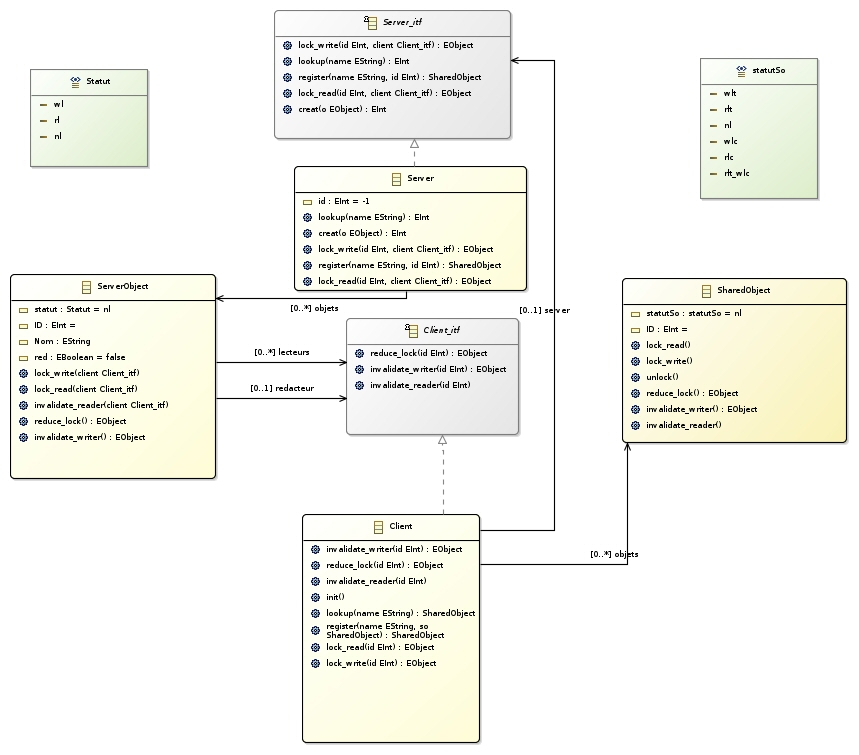
\includegraphics[scale=0.5]{diagram.jpg}
\end{center}
\end{figure}

Un client doit donc actionner la méthode $lock\_read$ avant de pouvoir lire, $lock\_read$ avant de pouvoir écrire, et $unlock$ pour débloquer l'objet lorsqu'il aura terminé. Nous allons expliquer l'implémentation de ces trois actions.

\subsection{Blocage en lecture}

La condition nécessaire pour pouvoir lire l'objet, est que personne n'écrive dessus ou n'ait l'objet en cache en écriture (statut $wlc$). \\
Lorsqu'on lance cette méthode sur un $SharedObject$, cette méthode va se propager, par le biais de la classe Client jusqu'au serveur, à qui on donnera l'id de l'objet, ainsi que le client qui veut lire dessus. Le serveur se charge de propager ce $lock\_read$ jusqu'au $ServerObject$ associé à l'id fourni. \\
Le $ServerObject$ associé possède les informations actuelles de l'objet, c'est à dire, son éventuel rédacteur (Client) ou ses éventuels lecteurs. On observe alors 3 situations: 
\begin{itemize}
\item Le $ServerObject$ possède un rédacteur qui est en train d'écrire. Dans ce cas, on lance un $reduce\_lock$ sur celui-ci. Cette méthode attendra alors que le rédacteur ait fini d'écrire (méthode synchronisée contenant wait), et le fera passer en $rlc$ directement après, au lieu de passer en $wlc$. Ainsi, le lecteur pourra accéder à l'objet, puisque celui-ci ne sera plus occupé en écriture. L'ancien rédacteur a donc l'objet en cache pour l'écriture, puisque le nouveau lecteur n'y fera aucune modifications. \\
Nous mettons également le $ServerObject$ concerné (on passe de $lw$ à $lr$, on ajoute le lecteur, ainsi que l'ancien rédacteur dans la collection de lecteurs (vide à ce moment là) et on met le rédacteur à {\bf null} et $red$ à \textbf{false}.
\item La dernière personne à a voir accédé à l'objet est un rédacteur. Il a donc encore l'objet en cache, et il faut le prévenir que quelqu'un veut accéder à la lecture. On répète donc la même manipulation que précédemment, en appliquant un $reduce\_lock$ sur l'ancien rédacteur, et en faisant les mises à jour nécessaires. 
\item Le $ServerObject$ est déjà occupé par d'autres personnes en lecture. Dans ce cas, il suffit de nous ajouter à la liste des lecteurs, et nous pouvons alors accéder à l'objet en lecture.\\\\
\end{itemize}

\textbf{Remarque:} Le serveur ne sait pas quand un rédacteur ou un lecteur arrête de lire ou d'écrire. Par conséquent, le fait qu'un rédacteur soit en train d'écrire ou ait déjà fini d'écrire ne change rien. Le $reduce\_lock$ attendra uniquement si le $SharedObject$ du rédacteur est encore en $wlt$. S'il est en $wlc$ (respectivement en $rlt\_wlc$ ), il passera en $nl$ (respectivement en $rlt$).\\\\

Une fois l'objet bloqué en lecture, on réalise un $notify()$, afin de réveiller d'éventuels lecteurs bloqués dans le $lock\_read$, puisqu'ils peuvent lire en même temps que nous. 

\newpage
\subsection{Blocage en écriture}

La condition nécessaire pour pouvoir écrire sur l'objet, est que personne ne soit en train d'écrire, ni de lire. Il faut donc que le $ServerObject$ ne possède pas de lecteur et que son rédacteur soit \textbf{null}.\\\\
On réalise donc les mêmes manipulations que précédemment lorsqu'on a un $lock\_write$ sur un $SharedOnject$, mais on l'applique différemment dans la méthode $lock\_read$ du $ServerObject$ concerné: 
\begin{itemize}
\item Si la dernière personne à avoir bloqué l'objet est un rédacteur, il faut l'invalider avec un $invalidate\_writer$. Cette méthode attend que cette personne ait fini d'écrire (que son $SharedObject$ soit passé en $wlc$, puis le fait passer en $nl$, puisque l'on va modifier l'objet. L'ancien rédacteur ne pourra donc plus écrire dessus ou le consulter.
\item Si l'objet est en train d'être lu par plusieurs personnes, et que d'autres personnes ont l'objet dans leur cache, il faut les invalider avec un $invalidate\_reader$. Cette méthode du $ServerObject$ va appliquer la méthode $invalidate\_reader$ de la classe Client sur chaque lecteur présent dans la collection de lecteurs du $ServerObject$. Chaque client appliquera donc cette méthode sur son $SharedObject$. Celle-ci attendra que le lecteur ait terminé de lire (lorsque le statut passera à $rlc$), et le fera passer en $nl$.\\
Une fois chaque lecteur invalidé, on vide la liste des lecteurs, et on affecte le rédacteur au client qui a lancé le $lock\_write$.
\end{itemize}

Une fois l'objet bloqué en écriture, personne ne pourra plus y accéder, et les personnes réalisant des lock sur les objets seront mises en attente, jusqu'à ce que le rédacteur réalise un unlock.
\newpage
\subsection{Libération des objets}

La méthode de déblocage est la même pour les lecteurs et les rédacteurs: 
\begin{itemize}
\item Si on est un lecteur, et qu'on a terminé de lire, on débloque notre $SharedObject$. Celui-ci va donc passer de $rlt$ à $rlc$, jusqu'à ce qu'un rédacteur ne le fasse passer à $nl$ (comme vu précédemment). Le lecteur n'est pas supprimé de la liste des lecteurs dans le $ServerObject$, puisqu'il possède toujours l'objet dans son cache, et est donc encore considéré comme un potentiel lecteur. On notifie également les personnes étant dans la file d'attente, afin qu'elles puissent accéder à la lecture ou à la lecture.
\item Si on est en écriture, on passe en $wlc$, mais le $ServerObject$ concerné possède toujours un rédacteur, jusqu'à la prochaine demande. On notifie alors les autres personnes étant en attente. Si ces personnes sont des lecteurs, et qu'elles accèdent à l'objet, nous pouvons toujours lire, puisque nous sommes la dernière personne à avoir modifié l'objet (on passe ainsi en $rlt\_wlc$ si on fait un $lock\_read$).
\end{itemize}

\textbf{Remarques:}
\begin{enumerate}
\item Les méthodes $lock\_read$ et $lock\_write$ du client sont synchronisées. Deux clients différents ne peuvent donc pas rentrer en même temps dans les deux. C'est cela qui permet le blocage des clients. 
\item Le réveil en chaîne des lecteurs ne se fait que dans l'ordre demandé. Si on a la séquence \textbf{R1 L1 L2 R2 L3}, et que \textbf{R1} libère l'objet, \textbf{L1, L2} seront libérés mais pas \textbf{L3}.
\end{enumerate}

\subsection{Test effectués}

L'application IRC fournie fonctionne correctement avec 4 IRC lancés en même temps. Chaque IRC possède toujours la dernière version de l'objet. \\
Nous avons également créé un IRCtest, qui permet ainsi de bloquer et débloquer les objets comme on le désire, et nous avons fait des essais pour voir comment étaient géré les attentes. Aucun interblocage n'a été détecté.
\begin{figure}[!h]
\begin{center}
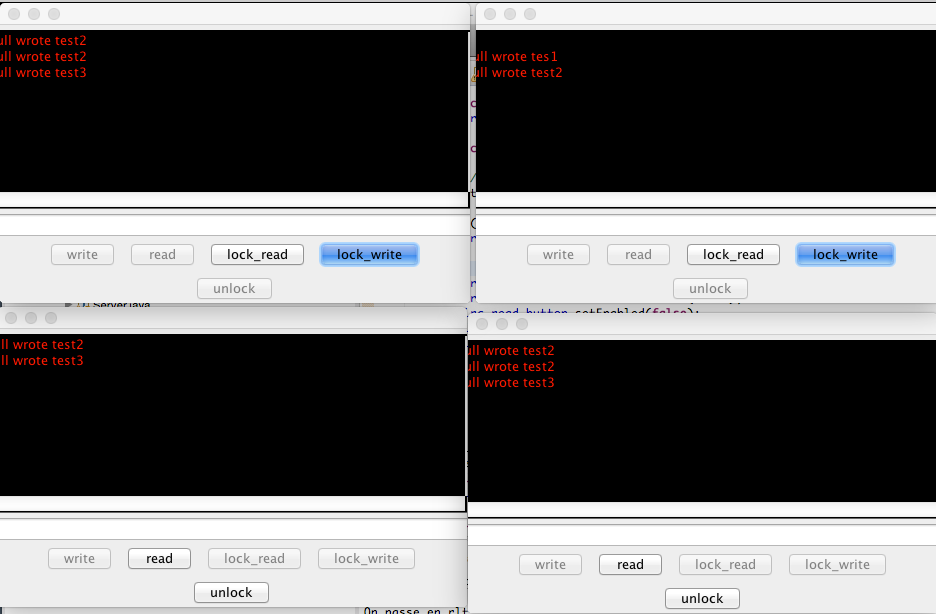
\includegraphics[scale=0.5]{IRCtes.png}
\end{center}
\end{figure}


\section{Implémentation des transaction}


L'étape 1 consistait en l’ajout d’une classe \textbf{Transaction}  permettant à l’application utilisateur (ici IRC) d’utiliser des transactions lors de ses appels en lecture/écriture, afin de se protéger d’une éventuelle coupure de courant ou autre erreur de la sorte.\\
En effet, lors d’un problème machine, sans transaction, la gestion de la concurrence des accès est perturbée, alors que la méthode abort() de la classe Transaction permet d’éviter tout problème en annulant les modifications faites par l’utilisateur et en libérant ensuite les verrous sur les objets concernés.\\\\

La classe Transaction dispose des méthodes suivantes :
\begin{itemize}
\item start() qui permet de définir une transaction comme la transaction courante (La classe Transaction dispose d’un attribut static \texttt{transationCourante}  qui gère cela).
\item commit() qui permet de valider les modifications de l’utilisateur (appel de $unlock()$ sur les $SharedObjects$) et de « fermer » la transaction (remettre l’attribut \texttt{transactionCourante} à null).
\item $abort()$ qui permet d’invalider les modifications de l’utilisateur et de « fermer » la transaction.
\item $getCurrentTransaction()$ qui retourne la transaction courante.\\\\
\end{itemize}


Il a également été nécessaire de modifier la classe $SharedObject$ pour que les méthodes $lock\_read()$ et $lock\_write()$ sauvegarde l’état de l’objet dans la transaction.\\ Et, évidemment, il a fallu changer la classe \texttt{Irc}  pour utiliser les transactions. Nous avons d’ailleurs choisi de laisser la possibilité à l’utilisateur de se servir ou non des transactions.


\section{Implémentation du générateur de Stubs}

L'étape 3 avait pour but de rendre l’utilisation des \textbf{SharedObjects}  plus discrète. En effet, avec l’utilisation de stub, l’utilisateur n’a plus à savoir se servir d’un   \textbf{SharedObject}.\\
Tout d’abord, nous avons dû crée un générateur de stub, qui, à partir d’une interface, pouvait créer une classe stub associée.
Ensuite, il a fallu modifier la classe \textbf{Client} afin qu’il ne crée non plus des $SharedObjects$ quelconques, mais des stub.\\ Il faut pour cela récupérer le nom de la classe stub puis récupérer son constructeur afin de créer une nouvelle instance de stub.\\
 Dans le cas du lookup du client, il faut pouvoir accéder à un objet afin de trouver le nom de la classe stub, c’est pourquoi nous avons rajouté une méthode $getObjectFromName()$ dans la classe \textbf{Server}. Cette méthode, comme son nom l’indique, retourne un objet contenu dans un \textbf{ServerObject}  possédant le nom donné en paramètre.
 
 \section*{Conclusion}
 
 Pour conclure, ce projet nous a permis d'illustrer le concept de la concurrence dans le domaine concret de l'objet partagé. Nous avons pu ainsi mêler les domaines de l'intergiciel (avec l'utilisation de serveurs RMI) et le système concurrents (avec les méthodes synchronisées). 
 
Le partage d'objets pourrait être plus permissif dans le cadre d'une application plus puissante, afin que tous les lecteurs et rédacteurs puissent y accéder en même temps (comme par exemple dans les document de google partagés sur le drive, où les modifications sont réalisées en direct pour chaque personne).   

\end{document}